\section{Results and Tests}
As described earlier, we decided to use a simlpe program that only copied the input registers into the output registers. This simplifies testing the power consumption exploring different techniques, like polling, interrupts and energy modes. 

	\subsection{Testing for correctness}
	\begin{figure}[t]
		\centerline{
			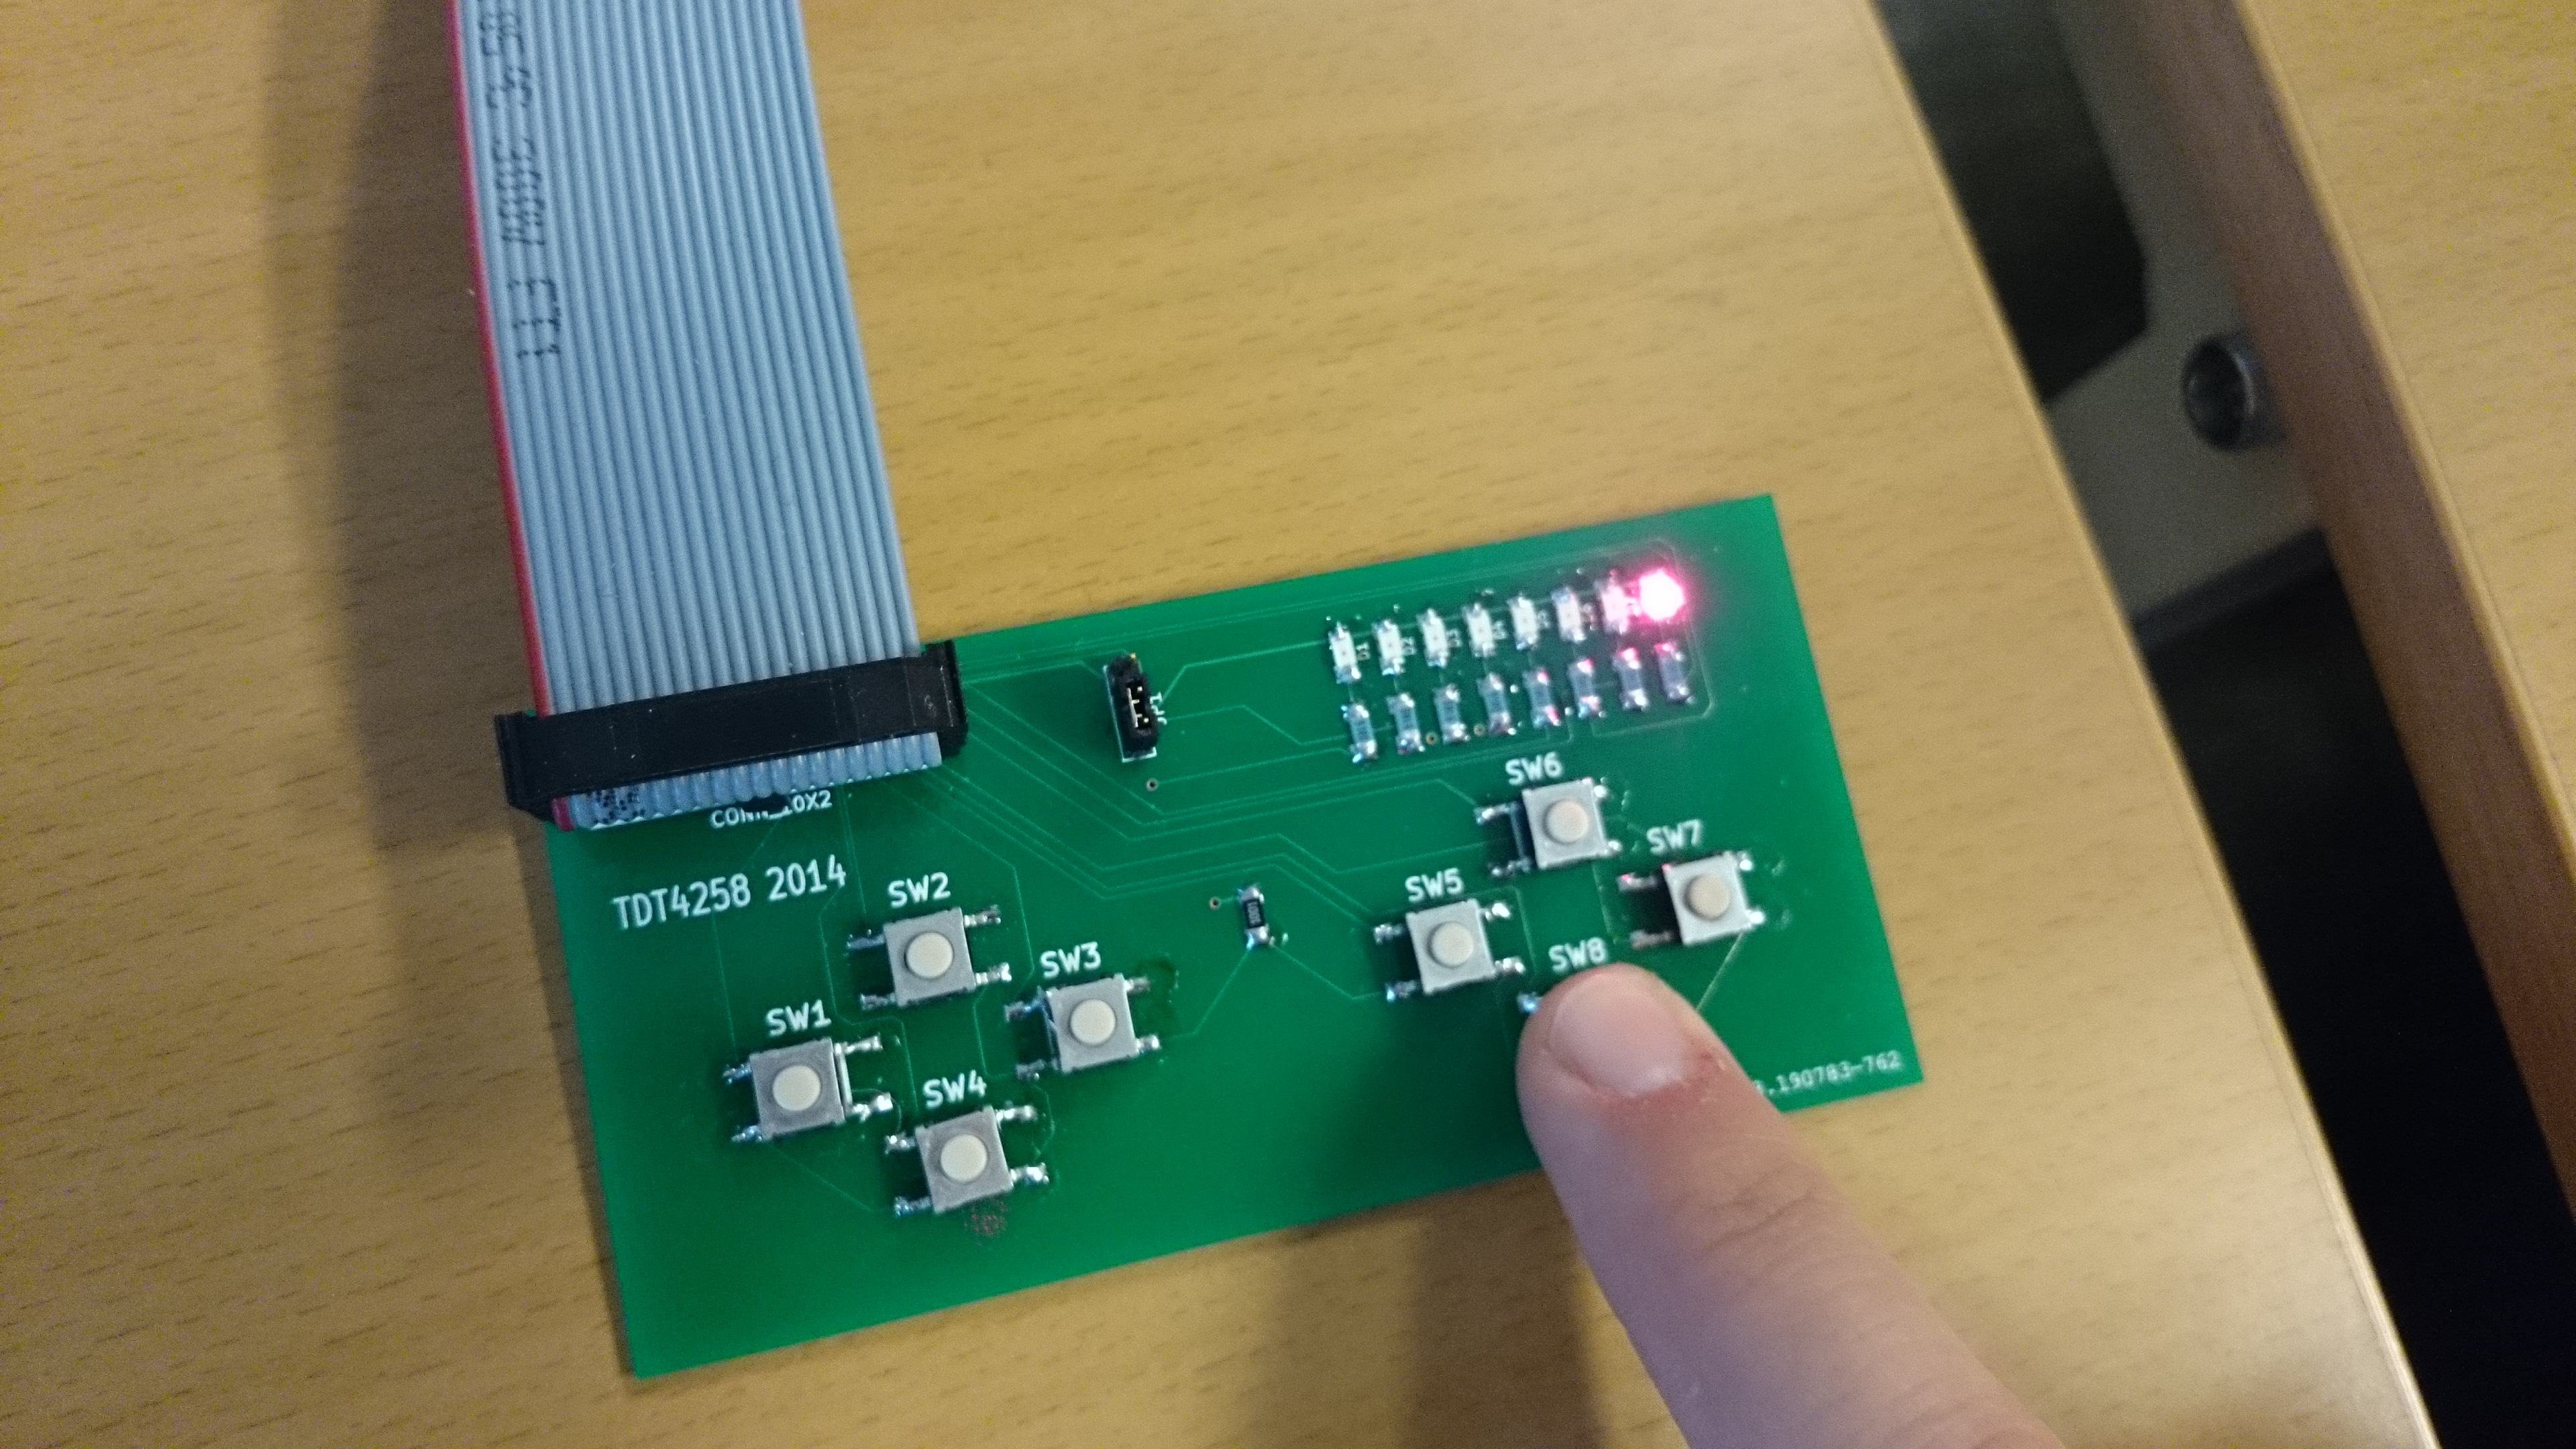
\includegraphics[width=0.5\textwidth]{img/test_correctness.jpg}
		}
		\caption{Verifying that the buttons and LEDs work correctly}
		\label{fig:test_correctness}
	\end{figure}
Testing the correctness for this simple program was easy. On every build, we confirmed that each button press lit the LED with the same number. Each LED should be on as long as the corresponding button is pressed. Se figure \ref{fig:test_correctness}.

	\subsection{Testing the energy effectiveness}
	In order to test the energy consumption of our system, we used the \emph{energyAware Profiler} provided by to us by Silicon Labs. We conducted the three following tests:

		\paragraph{Test 1 - No button press} 
		The system was run idle for ten seconds while the average amperage was measured. This test is important, because the system should consume less energy when it is idle.

		\paragraph{Test 2 - Button press}
		The system was run with buttons 1 and 8 held down continiously, which made LED 1 and 8 light during the whole test. The test was run for ten seconds, and average amperage was measured. We tested this, because we wanted to find out if the buttons consumed power, and if the interrupt routine worked as expected when the buttons were pressed down.

		\paragraph{Test 3 - Rapid button pressing}
		The system was run for ten seconds, with button 1 pressed twice each second. We ran this test to check the power consumption on the interrupt handling and wakeup procedures.
\\
\\
		All the tests was run without measuring the LED energy consumption. We used a handheld stopwatch for all the tests. The sample trace was dumped into a raw text file and further processed in a spreadsheet.


		\begin{figure}[t]

			\begin{tabular}{l | l | l | l | l | l}
				& Polling & Interrupts & Energy Mode 2 & Energy Mode 3 & Energy Mode 4 \\
				\hline
				Test 1 & $4.614mA$ & $3.350mA$ & $1.815\mu A$ & 1 & 70nA \\
				Test 2 & $4.497mA$ & $3.512mA$ & $160.0\mu A$ & 1 & - \\
				Test 3 & $4.618mA$ & $3.374mA$ & $20.07\mu A$ & 1 & - \\
			\end{tabular}
			\caption{Energy test results}
			\label{fig:test_results}
		\end{figure}

		\subsubsection{Polling}
		For the polling (section \ref{subsection:polling}), we measured a high amperage(around 4.5mA). With two of the buttens pressed down, the amperage was slightly reduced, and we do not know the reason for this. There was no noticable difference between test 1 and test 3. We expected to measure the same values for all three tests, since the system would keep on spinning in the same loop. The only thing that changes on button press, is the value on the registers.

		\subsubsection{Interrupts}
		We measured slightly lower power consumption on the code using interrupts (section \ref{subsection:interrupts}) than with the one using polling. Test 2 increased the amperage by approximately $0.2mA$. This was expected behaviour, as the buttons are active low, and use the internal pull up registers, and would drain a small amount of energy when pressed. Test 3 increased the power consumption with about $20\mu A$. We expected the system to use exacly the same amount of energy as with the polling because of the continious instruction execution (the system ran in a tight loop when idle), but this was obviously not the case.

		\subsubsection{EM2}
		Finally, we got some real power savings, three orders of magnitude lower than the previous tests. This is what we expected. We see that the pull-up resistors for the buttons still increase the energy consumption. The amperage was also higher for the rapid button press. We expected that the wakeup and interrupt procedure would consume some energy, but it is impossible to say whether the energy is consumed by this procedure or by the pull-up resistors.

		\subsubsection{EM3}
		The energy consumption in EM3 is the same as EM2. The only difference between EM2 and EM3 is that the low frequency oscilators are turned off in EM3\cite[p. 2]{enegy_optimization_application_note}. These were not in use in our application anyway.

		\subsubsection{EM4}
		\begin{figure}[t]
			\centerline{
				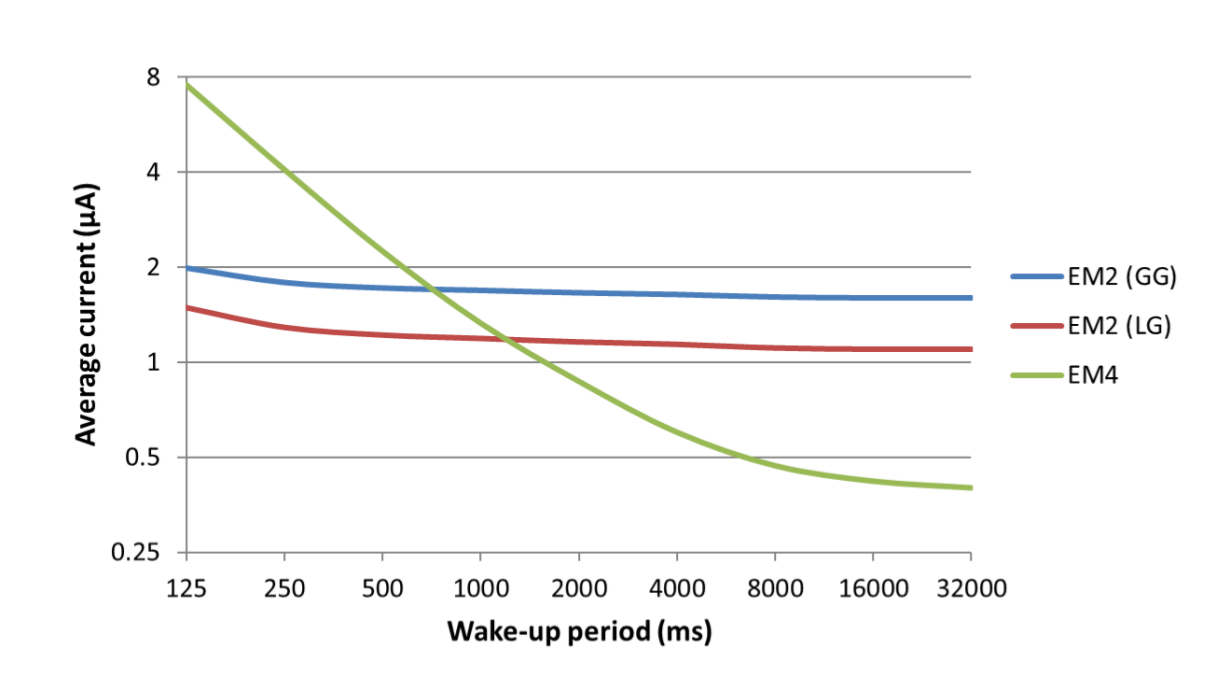
\includegraphics[width=0.7\textwidth]{img/em2vsem4.png}
			}
			\caption{Power consumption for periodic wake-up from EM2 vs EM4 (from \cite[p. 9]{energy_optimization_application_note})}
			\label{fig:em2vsem4}
			
		\end{figure}
		We tried out Energy Mode 4 (section \ref{subsubsection:em4}), but this would not pass the correctness test. The system was put to sleep and we found no way to wake it up again. The only way the system can return from EM4 pressing buttons on the gamepad is an interrupt via the GPIO wake-up pin \cite[p. 8]{reference_manual}, but this is not used in this application. Even though we were to find a way to make EM4 entry and return work, we have indications that this would not improve the energy efficiency of our system. The energy optimization application note from \emph{Silicon Labs} states that the average current is greater than EM2 if the system needs to wake up often (threshold around once a second, see figure \ref{fig:em2vsem4})  Either way, he EM4 energy efficiency is rather impressive; measured to only $70nA$!

